         \chapter{Number patterns}
    \setcounter{figure}{1}
    \setcounter{subfigure}{1}
    \label{d2d281c6991a4da87e4a19596c1ef625}
%          \section{ Introduction}
    \nopagebreak
            \label{m39364} $ \hspace{-5pt}\begin{array}{cccccccccccc}   
\includegraphics[width=0.75cm]{col11306.imgs/summary_fullmarks.png} &   
\includegraphics[width=0.75cm]{col11306.imgs/summary_video.png} &   \end{array} $ \hspace{2 pt}\raisebox{-5 pt}{} {(section shortcode: MG10022 )} \par 
%   
%     \label{m39364*cid1}
%             \subsection{ Introduction}
%             \nopagebreak
%             
      \label{m39364*id62175}In earlier grades you saw patterns in the form of pictures and numbers. In this chapter, we learn more about the mathematics of patterns. Patterns are recognisable as repetitive sequences and can be found in nature, shapes, events, sets of numbers and almost everywhere you care to look. For example, seeds in a sunflower, snowflakes, geometric designs on quilts or tiles, the number sequence $0;4;8;12;16;\mathrm{...}$.\par 
\label{m39364*secfhsst!!!underscore!!!id64}
        \begin{exercises}{Patterns }
         {
      \label{m39364*id62189}Can you spot any patterns in the following lists of numbers?\par 
      \label{m39364*id62194}\begin{enumerate}[noitemsep, label=\textbf{\arabic*}. ] 
            \label{m39364*uid1}\item $2;4;6;8;10;...$\label{m39364*uid2}\item $1;2;4;7;11;...$
\label{m39364*uid3}\item $1;4;9;16;25;...$
\label{m39364*uid4}\item $5;10;20;40;80;...$
\end{enumerate}
}
    \label{m39364*cid2}
            \section{Number Pattern Examples}
            \nopagebreak
            \label{m39364*id62635}Numbers can have interesting patterns. Here we list the most common patterns and how they are made.\par 
      \label{m39364*id62640}Examples:\par 
      \label{m39364*id62643}\begin{enumerate}[noitemsep, label=\textbf{\arabic*}. ] 
            \label{m39364*uid5}\item $1;4;7;10;13;16;19;22;25;...$
This sequence has a difference of 3 between each number.
The pattern is continued by adding 3 to the last number each time.
\label{m39364*uid6}\item $3;8;13;18;23;28;33;38;...$
This sequence has a difference of 5 between each number.
The pattern is continued by adding 5 to the last number each time.
\label{m39364*uid7}\item $2;4;8;16;32;64;128;256;...$
This sequence has a factor of 2 between each number.
The pattern is continued by multiplying the last number by 2 each time.
\label{m39364*uid8}\item $3;9;27;81;243;729;2187;...$
This sequence has a factor of 3 between each number.
The pattern is continued by multiplying the last number by 3 each time.
\end{enumerate}
      \label{m39364*uid9}
           \subsection*{ Special Sequences}
            \nopagebreak
            \label{m39364*uid10}
            \subsubsection*{ Triangular Numbers}
            \nopagebreak
          \label{m39364*id62915}
            $1;3;6;10;15;21;28;36;45;...$
          \par 
          \label{m39364*id62968}This sequence is generated from a pattern of dots which form a triangle.
By adding another row of dots (with one more dot in each row than in the previous row) and counting all the dots, we can find the next number of the sequence.\par 
        \label{m39364*uid11}
            \subsubsection*{ Square Numbers}
            \nopagebreak
          \label{m39364*id62984}
            $1;4;9;16;25;36;49;64;81;...$
          \par 
          \label{m39364*id63037}The next number is made by squaring the number of the position in the pattern.
The second number is 2 squared (${2}^{2}\phantom{\rule{3.33333pt}{0ex}}or\phantom{\rule{3.33333pt}{0ex}}2\ensuremath{\times}2$ \hspace{1ex}). 
The seventh number is 7 squared (${7}^{2}\phantom{\rule{3.33333pt}{0ex}}or\phantom{\rule{3.33333pt}{0ex}}7\ensuremath{\times}7$  \hspace{1ex} ) etc.\par 
        \label{m39364*uid12}
            \subsubsection*{ Cube Numbers}
            \nopagebreak
          \label{m39364*id63115}
            $1;8;27;64;125;216;343;512;729;...$
          \par 
          \label{m39364*id63168}The next number is made by cubing the number of the position in the pattern.
The second number is 2 cubed (${2}^{3}\phantom{\rule{3.33333pt}{0ex}}or\phantom{\rule{3.33333pt}{0ex}}2\ensuremath{\times}2\ensuremath{\times}2$ \hspace{1ex}).
The seventh number is 7 cubed (${7}^{3}\phantom{\rule{3.33333pt}{0ex}}or\phantom{\rule{3.33333pt}{0ex}}7\ensuremath{\times}7\ensuremath{\times}7$\hspace{2ex}) etc.\par 
        \label{m39364*uid13}
            \subsubsection*{ Fibonacci Numbers}
            \nopagebreak
          \label{m39364*id63254}
            $0;1;1;2;3;5;8;13;21;34;...$
          \par 
          \label{m39364*id63490}The next number is found by adding the two numbers before it together.
The 2 is found by adding the two numbers in front of it ($1+1$).
The 21 is found by adding the two numbers in front of it ($8+13$).
The next number in the sequence above would be 55 ($21+34$).\par 
          \label{m39364*id63538}Can you figure out the next few numbers?\par 
\label{m39364*eip-450}
    \setcounter{subfigure}{0}
	\begin{figure}[H] % horizontal\label{m39364*numberpatterns-1}
    \textnormal{Khan Academy video on Number Patterns - 1}\vspace{.1in} \nopagebreak
  \label{m39364*yt-media1}\label{m39364*yt-video1}
            \raisebox{-5 pt}{ 
\includegraphics[width=0.5cm]{col11306.imgs/summary_www.png}} { (Video:  MG10023 )}
      \vspace{2pt}
    \vspace{.1in}
 \end{figure}       
% \par \label{m39364*secfhsst!!!underscore!!!id280}\vspace{.5cm} 
%       \noindent
%       \hspace*{-30pt}
\includegraphics[width=0.5in]{col11306.imgs/pspencil2.png}   \raisebox{25mm}{   
%       \begin{mdframed}[linewidth=4, leftmargin=40, rightmargin=40]  
\begin{wex}{Study Table}{Say you and 3 friends decide to study for Maths, and you are seated at a square table. A few minutes later, 2 other friends join you and would like to sit at your table and help you study. Naturally, you move another table and add it to the existing one. Now 6 of you sit at the table. Another 2 of your friends join your table, and you take a third table and add it to the existing tables. Now 8 of you can sit comfortably.
\begin{figure}[H]
\begin{center}
\begin{pspicture}(0,0)(9.6,1.8)
%\psgrid[gridcolor=lightgray]
\psframe(0.4,0.4)(1.4,1.4)
\psframe(0,0.6)(0.2,1.2)
\psframe(0.6,0)(1.2,0.2)
\psframe(0.6,1.6)(1.2,1.8)
\psframe(1.6,0.6)(1.8,1.2)
\rput(2.4,0){\psframe(0.4,0.4)(1.4,1.4)
\psframe(0,0.6)(0.2,1.2)
\psframe(0.6,0)(1.2,0.2)
\psframe(0.6,1.6)(1.2,1.8)}
\rput(3.4,0){\psframe(0.4,0.4)(1.4,1.4)
\psframe(0.6,0)(1.2,0.2)
\psframe(0.6,1.6)(1.2,1.8)
\psframe(1.6,0.6)(1.8,1.2)}
\rput(5.8,0){\psframe(0.4,0.4)(1.4,1.4)
\psframe(0,0.6)(0.2,1.2)
\psframe(0.6,0)(1.2,0.2)
\psframe(0.6,1.6)(1.2,1.8)}
\rput(6.8,0){\psframe(0.4,0.4)(1.4,1.4)
\psframe(0.6,0)(1.2,0.2)
\psframe(0.6,1.6)(1.2,1.8)}
\rput(7.8,0){\psframe(0.4,0.4)(1.4,1.4)
\psframe(0.6,0)(1.2,0.2)
\psframe(0.6,1.6)(1.2,1.8)
\psframe(1.6,0.6)(1.8,1.2)}
\end{pspicture}
\caption{Two more people can be seated for each table added.}
\label{fig:mp:s:arithmetictables}
\end{center}
\end{figure}
Examine how the number of people sitting is related to the number of tables.}
{
\westep{Tabulate a few terms to see if there is a pattern}
\begin{center}
\begin{tabular}{|c|l|}\hline
\hline \textbf{Number of Tables}, $n$ & \textbf{Number of people seated}\\\hline
\hline 1 & $4 = 4$\\
\hline 2 & $4 + 2 = 6$\\
\hline 3 & $4 + 2 + 2 = 8$\\
\hline 4 & $4 + 2 + 2 + 2 = 10$ \\
\hline \vdots & \qquad \qquad \quad \vdots\\
\hline $n$ & $4 + 2 + 2 + 2 + \ldots + 2 $\\
\hline\hline
\end{tabular}
\end{center}
\westep{Describe the pattern}
We can see that for 3 tables we can seat 8 people, for 4 tables we can seat 10 people and so on. We started out with 4 people and added two each time. Thus, for each table added, the number of persons increased by 2.}%\end{wex}
}
\end{wex}
    
%     \noindent
%   \label{m39364**end}
         \section{ Notation}
    \nopagebreak
            \label{m39362} $ \hspace{-5pt}\begin{array}{cccccccccccc}   
\includegraphics[width=0.75cm]{col11306.imgs/summary_fullmarks.png} &   
\includegraphics[width=0.75cm]{col11306.imgs/summary_video.png} &   \end{array} $ \hspace{2 pt}\raisebox{-5 pt}{} {(section shortcode: MG10024 )} \par 
%   
%     \label{m39362*cid4}
%             \subsection{ Notation}
%             \nopagebreak
    \setcounter{subfigure}{0}
	\begin{figure}[H] % horizontal\label{m39362*numberpatterns-3}
    \textnormal{Khan Academy video on Number Patterns}\vspace{.1in} \nopagebreak
  \label{m39362*yt-media3}\label{m39362*yt-video3}
            \raisebox{-5 pt}{ 
\includegraphics[width=0.5cm]{col11306.imgs/summary_www.png}} { (Video:  MG10025 )}
      \vspace{2pt}
    \vspace{.1in}
 \end{figure}       
      \label{m39362*eip-149}The ${n}^{\mathrm{th}}$-term of a sequence is written as ${a}_{n}$. So for example, the ${1}^{\mathrm{st}}$-term of a sequence is ${a}_{1}$, the ${10}^{\mathrm{th}}$-term is ${a}_{10}$.\par \label{m39362*id63992}A sequence does not have to follow a pattern but when it does, we can often write down a formula to calculate the ${n}^{\mathrm{th}}$-term, ${a}_{n}$. In the sequence\par 
      \label{m39362*id64025}\nopagebreak\noindent{}
        
    \begin{equation}
    1;4;9;16;25;...\tag{2.1}
      \end{equation}
      \label{m39362*id64058}where the sequence consists of the squares of integers, the formula for the ${n}^{\mathrm{th}}$-term is\par 
      \label{m39362*uid15}\nopagebreak\noindent{}
        
    \begin{equation}
    \begin{array}{cc}\hfill {a}_{n}={n}^{2}\end{array}\tag{2.2}
      \end{equation}
      \label{m39362*id64117}You can check this by looking at:\par 
      \label{m39362*id64122}\nopagebreak\noindent{}
        
    \begin{equation}
    \begin{array}{ccc}\hfill {a}_{1}& =& {1}^{2}\phantom{\rule{0.277778em}{0ex}}=\phantom{\rule{0.277778em}{0ex}}1\hfill \\ \hfill {a}_{2}& =& {2}^{2}\phantom{\rule{0.277778em}{0ex}}=\phantom{\rule{0.277778em}{0ex}}4\hfill \\ \hfill {a}_{3}& =& {3}^{2}\phantom{\rule{0.277778em}{0ex}}=\phantom{\rule{0.277778em}{0ex}}9\hfill \\ \hfill {a}_{4}& =& {4}^{2}\phantom{\rule{0.277778em}{0ex}}=\phantom{\rule{0.277778em}{0ex}}16\hfill \\ \hfill {a}_{5}& =& {5}^{2}\phantom{\rule{0.277778em}{0ex}}=\phantom{\rule{0.277778em}{0ex}}25\hfill \\ \hfill ...\end{array}\tag{2.3}
      \end{equation}
      \label{m39362*id64323}Therefore, using (2.2), we can generate a pattern, namely squares of integers.\par 
\label{m39362*eip-695}We can also define the common difference for a pattern. \vspace{\rubberspace}\par
%         \label{m39362*id743}\begin{definition}
% 	  \begin{tabular*}{15 cm}{m{15 mm}m{}}
% 	\hspace*{-50pt}  
\includegraphics[width=0.5in]{col11306.imgs/psflag2.png}   & 
\Definition{   Common difference} {The common difference is the difference between successive terms and is denoted by d. } 
%       \end{tabular*}
%       \end{definition}
For example, consider the sequence $10;7;4;1;\mathrm{...}$ . To find the common difference, we simply subtract each successive term:
\label{m39362*id872}\nopagebreak\noindent{}

    \begin{equation}
    \begin{array}{ccc}7-10& =& -3\\ 4-7& =& -3\\ 1-4& =& -3\end{array}\tag{2.4}
      \end{equation}
 \par \par
%             \label{m39362*secfhsst!!!underscore!!!id574}\vspace{.5cm} 
%       \noindent
%       \hspace*{-30pt}
\includegraphics[width=0.5in]{col11306.imgs/pspencil2.png}   \raisebox{25mm}{   
%       \begin{mdframed}[linewidth=4, leftmargin=40, rightmargin=40]  
%       
\begin{wex}{Study Table continued ....}{As before, you and 3 friends are studying for Maths, and you are seated at a square table. A few minutes later, 2 other friends join you move another table and add it to the existing one. Now 6 of you sit at the table. Another 2 of your friends join your table, and you take a third table and add it to the existing tables. Now 8 of you sit comfortably as illustrated:
\begin{figure}[H]
\begin{center}
\begin{pspicture}(0,0)(9.6,1.8)
%\psgrid[gridcolor=lightgray]
\psframe(0.4,0.4)(1.4,1.4)
\psframe(0,0.6)(0.2,1.2)
\psframe(0.6,0)(1.2,0.2)
\psframe(0.6,1.6)(1.2,1.8)
\psframe(1.6,0.6)(1.8,1.2)
\rput(2.4,0){\psframe(0.4,0.4)(1.4,1.4)
\psframe(0,0.6)(0.2,1.2)
\psframe(0.6,0)(1.2,0.2)
\psframe(0.6,1.6)(1.2,1.8)}
\rput(3.4,0){\psframe(0.4,0.4)(1.4,1.4)
\psframe(0.6,0)(1.2,0.2)
\psframe(0.6,1.6)(1.2,1.8)
\psframe(1.6,0.6)(1.8,1.2)}
\rput(5.8,0){\psframe(0.4,0.4)(1.4,1.4)
\psframe(0,0.6)(0.2,1.2)
\psframe(0.6,0)(1.2,0.2)
\psframe(0.6,1.6)(1.2,1.8)}
\rput(6.8,0){\psframe(0.4,0.4)(1.4,1.4)
\psframe(0.6,0)(1.2,0.2)
\psframe(0.6,1.6)(1.2,1.8)}
\rput(7.8,0){\psframe(0.4,0.4)(1.4,1.4)
\psframe(0.6,0)(1.2,0.2)
\psframe(0.6,1.6)(1.2,1.8)
\psframe(1.6,0.6)(1.8,1.2)}
\end{pspicture}
\caption{Two more people can be seated for each table added.}
\label{fig:mp:s:arithmetictables2}
\end{center}
\end{figure}
Find the expression for the number of people seated at $n$ tables. Then, use the general formula to determine how many people can sit around 12 tables and how many tables are needed for 20 people.}{
\westep{Tabulate a few terms to see if there is a pattern}
\begin{center}
\begin{tabular}{|c|l|c|}\hline
\hline \textbf{Number of Tables}, $n$ & \textbf{Number of people seated} & \textbf{Formula}\\\hline
\hline 1 & $4 = 4$ & $= 4 + 2 \cdot(0)$ \\
\hline 2 & $4 + 2 = 6$ & $= 4 + 2 \cdot(1)$ \\
\hline 3 & $4 + 2 + 2 = 8$ & $= 4 + 2 \cdot(2)$ \\
\hline 4 & $4 + 2 + 2 + 2 = 10$ & $= 4 + 2\cdot(3)$ \\
\hline \vdots & \qquad \qquad \quad \vdots & \vdots \\
\hline $n$ & $4 + 2 + 2 + 2 + \ldots + 2 $ & \: \: \: $= 4 + 2\cdot (n-1)$\\
\hline\hline
\end{tabular}
\end{center}

\westep{Describe the pattern}
The number of people seated at $n$ tables is:
\nequ{a_n=4 + 2\cdot (n-1)}

\westep{Calculate the $12^{\mathrm{th}}$ term}
Considering the example from the previous section, how many people can sit around, say, 12 tables? We are looking for $a_{12}$, that is, where $n = 12$:
\begin{eqnarray*}
a_n &=& a_1 + d \cdot (n - 1) \\
a_{12} &=& 4 + 2 \cdot (12 - 1) \\
&=& 4 + 2(11) \\
&=& 4 + 22 \\
&=& 26
\end{eqnarray*}

\westep{Calculate the number of terms if $a_n=20$}
\begin{eqnarray*}
a_n &=& a_1 + d \cdot (n - 1) \\
20 &=& 4 + 2 \cdot (n - 1) \\
20 - 4 &=& 2 \cdot (n - 1) \\
16 \div 2 &=& n - 1 \\
8 + 1 &=& n \\
n &=& 9
\end{eqnarray*}
\westep{Final Answer}
26 people can be seated at 12 tables and 9 tables are needed to seat 20 people.}%\end{wex}

}
    \end{wex}
%     \end{mdframed}
%     }
    \noindent
      \label{m39362*id65378}It is also important to note the difference between $n$ and ${a}_{n}$. $n$ can be compared to a place holder, while ${a}_{n}$ is the value at the place ``held'' by $n$. Like our ``Study Table'' example above, the first table (Table 1) holds 4 people. Thus, at place $n=1$, the value of ${a}_{1}=4$ and so on:\par 
    
\begin{center}
\begin{tabular}{|c|c|c|c|c|c|}
\hline $n$ & 1 & 2 & 3 & 4 & \ldots \\
\hline $a_n$ & 4 & 6 & 8 & 10 & \ldots \\
\hline
\end{tabular}
\end{center}
\label{m39362*secfhsst!!!underscore!!!id1060}
          \begin{exercises}{General Formula }
           { \nopagebreak
      \label{m39362*id65612}\begin{enumerate}[noitemsep, label=\textbf{\arabic*}. ] 
            \label{m39362*uid17}\item Find the general formula for the following sequences and then find ${a}_{10}$, ${a}_{50}$ and ${a}_{100}$:
\label{m39362*id65671}\begin{enumerate}[noitemsep, label=\textbf{\alph*}. ] 
            \label{m39362*uid18}\item $2;5;8;11;14;...$\label{m39362*uid19}\item $0;4;8;12;16;...$\label{m39362*uid20}\item $2;-1;-4;-7;-10;...$\end{enumerate}
        \label{m39362*uid21}\item The general term has been given for each sequence below. Work out the missing terms.
\label{m39362*id65820}\begin{enumerate}[noitemsep, label=\textbf{\alph*}. ] 
            \label{m39362*uid22}\item $0;3;...;15;24$ ~~~~~~${n}^{2}-1$\label{m39362*uid23}\item $3;2;1;0;...;-2$ ~~~~~~$-n+4$\label{m39362*uid24}\item $-11;...;-7;...;-3$ ~~~~~~$-13+2n$\end{enumerate}
        \end{enumerate}}
      \label{m39362*uid25}
            \section{ Patterns and Conjecture}
            \nopagebreak
        \label{m39362*eip-362}
    \setcounter{subfigure}{0}
	\begin{figure}[H] % horizontal\label{m39362*numberpatterns-2}
    \textnormal{Khan Academy video on Number Patterns - 2}\vspace{.1in} \nopagebreak
  \label{m39362*yt-media2}\label{m39362*yt-video2}
            \raisebox{-5 pt}{ 
\includegraphics[width=0.5cm]{col11306.imgs/summary_www.png}} { (Video:  MG10026 )}
      \vspace{2pt}
    \vspace{.1in}
 \end{figure}       \par \label{m39362*id66036}In mathematics, a conjecture is a mathematical statement which appears to be true, but has not been formally proven to be true. A conjecture can be seen as an educated guess or an idea about a pattern. A conjecture can be thought of as the mathematicians way of saying I believe that this is true, but I have no proof.\par 
        \label{m39362*id66042}For example: Make a \textbf{conjecture} about the next number based on the pattern $2;6;11;17;...$\par 
        \label{m39362*id66085}The numbers increase by 4, 5, and 6.\par 
        \label{m39362*id66090}\textbf{Conjecture:} The next number will increase by 7. So, it will be $17+7$ or 24.\par 
\label{m39362*secfhsst!!!underscore!!!id1075}\vspace{.5cm} 
%       \noindent
%       \hspace*{-30pt}
\includegraphics[width=0.5in]{col11306.imgs/pspencil2.png}   \raisebox{25mm}{   
%       \begin{mdframed}[linewidth=4, leftmargin=40, rightmargin=40]  
      \begin{wex}{ Number patterns }
   {Consider the following pattern: 
  
          
    \begin{equation}
    \begin{array}{ccc}\hfill {1}^{2}+1& =& {2}^{2}-2\hfill \\ \hfill {2}^{2}+2& =& {3}^{2}-3\hfill \\ \hfill {3}^{2}+3& =& {4}^{2}-4\hfill \\ \hfill {4}^{2}+4& =& {5}^{2}-5\hfill \end{array}\tag{2.8}
      \end{equation}
        \label{m39362*id66291}\begin{enumerate}[noitemsep, label=\textbf{\arabic*}. ] 
            \leftskip=20pt\rightskip=\leftskip\label{m39362*uid26}\item Add another two rows to the end of the pattern.
\label{m39362*uid27}\item Make a conjecture about this pattern. Write your conjecture in words.
\label{m39362*uid28}\item Generalise your conjecture for this pattern (in other words, write your conjecture algebraically).
\label{m39362*uid29}\item Prove that your conjecture is true.
\end{enumerate}}{
%         \vspace{5pt}
%         \label{m39362*solfhsst!!!underscore!!!id1196}\noindent\textbf}{ \label{m39362*listfhsst!!!underscore!!!id1196}\begin{enumerate}[noitemsep, label=\textbf{Step} \textbf{\arabic*}. ] 
% %             \leftskip=20pt\rightskip=\leftskip\item  
%         \label{m39362*id66367}\nopagebreak\noindent{}
%           
\westep{}  
  \begin{equation}
    \begin{array}{cc}\hfill {5}^{2}+5={6}^{2}-6\\ \hfill {6}^{2}+6={7}^{2}-7\end{array}\tag{2.9}
      \end{equation}
        \westep{}  
        \label{m39362*id66445}Squaring a number and adding the same number gives the same result as squaring the next number and subtracting that number.\par 
        \westep{}
        \label{m39362*id66453}We have chosen to use $x$ here. You could choose any letter to generalise the pattern.\par 
        \label{m39362*id66467}\nopagebreak\noindent{}
          
    \begin{equation}
    {x}^{2}+x={\left(x+1\right)}^{2}-\left(x+1\right)\tag{2.10}
      \end{equation}
        \westep{}  
%         \label{m39362*id66525}\nopagebreak\noindent{}
          
    \begin{equation}
    \mathrm{Left\; side}:\phantom{\rule{3.33333pt}{0ex}}{x}^{2}+x\tag{2.11}
      \end{equation}
        \label{m39362*id66572}\nopagebreak\noindent{}
          
    \begin{equation}
    \mathrm{Right\; side}:\phantom{\rule{3.33333pt}{0ex}}{\left(x+1\right)}^{2}-\left(x+1\right)\tag{2.12}
      \end{equation}
        \label{m39362*id66641}\nopagebreak\noindent{}
    \begin{equation}
    \begin{array}{ccc}\mathrm{Right\; side}\hfill & =& {x}^{2}+2x+1-x-1\hfill \\ & =& {x}^{2}+x\hfill \\ & =& \mathrm{Left\; side}\hfill \\ \therefore \phantom{\rule{3.33333pt}{0ex}}{x}^{2}+x\hfill & =& {\left(x+1\right)}^{2}-\left(x+1\right)\hfill \end{array}\tag{2.13}
      \end{equation}
     
}
    \end{wex}
    \end{mdframed}   
    \noindent
    \label{m39362*eip-817}
            \section{ Summary}
            \nopagebreak
            \label{m39362*uid08213123}\begin{itemize}[noitemsep]
            \item There are several special sequences of numbers: \label{m39362*uid8271312}\begin{itemize}[noitemsep]
            \item Triangular numbers  $1;3;6;10;15;21;28;36;45;...$\item Square numbers $1;4;9;16;25;36;49;64;81;...$\item Cube numbers $1;8;27;64;125;216;343;512;729;...$\item Fibonacci numbers $0;1;1;2;3;5;8;13;21;34;...$\end{itemize}
        \item We represent the ${n}^{\mathrm{th}}$-term with the notation ${a}_{n}$\item We can define the common difference of a sequence as the difference between successive terms.\item We can work out a general formula for each number pattern and use that to predict what any number in the pattern will be.\end{itemize}
        \label{m39362*cid5}
           

\begin{eocexercises}{End of Chapter Exercises}
            \nopagebreak
      \label{m39362*id66867}\begin{enumerate}[noitemsep, label=\textbf{\arabic*}. ] 
            \label{m39362*uid30}\item Find the ${n}^{\mathrm{th}}$ term for: $3,7,11,15,...$
        \label{m39362*uid31}\item Find the general term of the following sequences:
\label{m39362*id66935}\begin{enumerate}[noitemsep, label=\textbf{\alph*}. ] 
            \label{m39362*uid32}\item $-2;1;4;7;...$\label{m39362*uid33}\item $11;15;19;23;...$\label{m39362*uid34}\item sequence with ${a}_{3}=7$ and ${a}_{8}=15$\label{m39362*uid35}\item sequence with ${a}_{4}=-8$ and ${a}_{10}=10$\end{enumerate}
        \label{m39362*uid36}\item The seating in a section of a sports stadium can be arranged so the first row has 15 seats, the second row has 19 seats, the third row has 23 seats and so on. Calculate how many seats are in the row 25.
        \label{m39362*uid43}\item A single square is made from 4 matchsticks. Two squares in a row need 7 matchsticks and 3 squares in a row need 10 matchsticks. Determine:
\label{m39362*id67360}\begin{enumerate}[noitemsep, label=\textbf{\alph*}. ] 
            \label{m39362*uid44}\item the first term
\label{m39362*uid45}\item the common difference
\label{m39362*uid46}\item the formula for the general term
\label{m39362*uid47}\item how many matchsticks are in a row of 25 squares
\end{enumerate}
    \setcounter{subfigure}{0}
	\begin{figure}[H] % horizontal\label{m39362*id67417}
    \begin{center}
    \label{m39362*id67417!!!underscore!!!media}\label{m39362*id67417!!!underscore!!!printimage}
%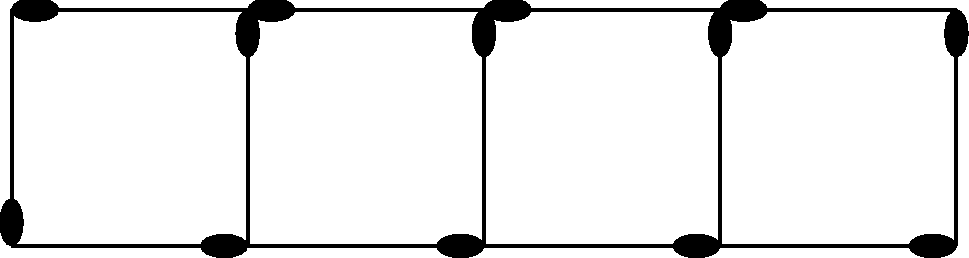
\includegraphics[width=300px]{col11306.imgs/m39362_MG10C7_004.png} % m39362;MG10C7\_004.png;;;6.0;8.5;
\begin{pspicture}(0,0)(8,2)
%\psgrid[gridcolor=gray]
\def\match{\psline(0,0)(2,0)\psellipse*(1.8,0)(0.2,0.1)}
\rput(0,0){\match}
\rput{90}(2,0){\match}
\rput{180}(2,2){\match}
\rput{270}(0,2){\match}
\rput(2,0){\rput(0,0){\match}
\rput{90}(2,0){\match}
\rput{180}(2,2){\match}}
\rput(4,0){\rput(0,0){\match}
\rput{90}(2,0){\match}
\rput{180}(2,2){\match}}
\rput(6,0){\rput(0,0){\match}
\rput{90}(2,0){\match}
\rput{180}(2,2){\match}}
\end{pspicture}

      \vspace{2pt}
    \vspace{.1in}
    \end{center}
 \end{figure}       
        \label{m39362*uid48}\item You would like to start saving some money, but because you have never tried to save money before, you have decided to start slowly. At the end of the first week you deposit R5 into your bank account. Then at the end of the second week you deposit R10 into your bank account. At the end of the third week you deposit R15. After how many weeks do you deposit R50 into your bank account?
        \label{m39362*uid49}\item A horizontal line intersects a piece of string at
four points and divides it into five parts, as shown below.
    \setcounter{subfigure}{0}
	\begin{figure}[H] % horizontal\label{m39362*id67455}
    \begin{center}
    \label{m39362*id67455!!!underscore!!!media}\label{m39362*id67455!!!underscore!!!printimage}
%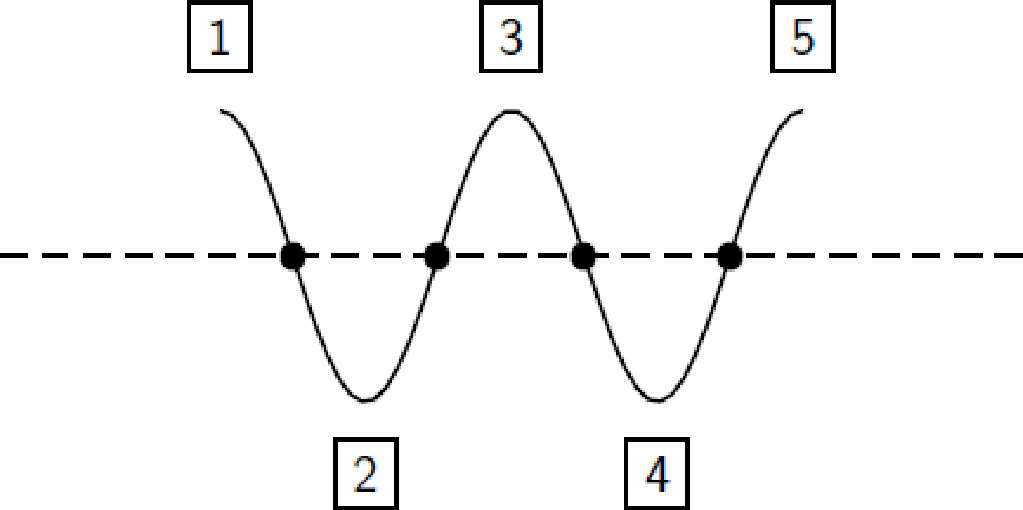
\includegraphics[width=250px]{col11306.imgs/m39362_MG10C7_005.png} % m39362;MG10C7\_005.png;;;6.0;8.5;
\begin{pspicture}(-1,-2)(6,2)
%\psgrid[gridcolor=gray]
\psplot[xunit=0.00556]{90}{810}{x sin}
\psline[linestyle=dashed](-1,0)(6,0)
\psdots[dotsize=5pt](1,0)(2,0)(3,0)(4,0)
\rput(0.5,1.5){\psframebox{1}}
\rput(1.5,-1.5){\psframebox{2}}
\rput(2.5,1.5){\psframebox{3}}
\rput(3.5,-1.5){\psframebox{4}}
\rput(4.5,1.5){\psframebox{5}}
\end{pspicture}
    \end{center}
 \end{figure}       
If the piece of string is intersected in this way by 19 parallel
lines, each of which intersects it at four points, find the number
of parts into which the string will be divided.
        \end{enumerate}
  \label{m39362**end}
  \label{d2d281c6991a4da87e4a19596c1ef625**end}
\par \raisebox{-5 pt}{
\includegraphics[width=0.5cm]{col11306.imgs/summary_www.png}} Find the answers with the shortcodes:
 \par \begin{tabular}[h]{cccccc}
 (1.) lcq  &  (2.) lcl  &  (3.) lci  &  (4.) lOe  &  (5.) lcO  &  (6.) lcc  & \end{tabular}
\end{eocexercises}
